\documentclass{beamer}
\usepackage[utf8]{inputenc}
\usepackage{hyperref}
\usepackage{multicol}
\usepackage{hyperref}
\usepackage{graphicx}
\usepackage{booktabs}
\usepackage[font={small,it},labelfont=bf]{caption}
\hypersetup{
    colorlinks=true,
    urlcolor={blue!40!black},
    linkcolor={red!50!black}
}

\inputencoding{utf8}

\mode<presentation> {
    \usetheme{Madrid}
}

\title{Metodologias de desarollo}
\author{Prof. Ernesto Rodriguez}
\institute{
    Universidad del Itsmo \\
    \medskip \textit{erodriguez@unis.edu.gt}
}

\date[\today]{}

\begin{document}

\begin{frame}
\titlepage
\end{frame}

\begin{frame}
    \frametitle{Metodologia de desarrollo}
    \begin{itemize}
        \item{Conjunto de practicas y lineamientos para
        estructurar el proceso de desarrollo.}
        \item{Existen varias opciones, cada una con ventajas
        y desventajas seg\'un la naturaleza del pryecto.}
        \item{Muchas metodologias tienen herramientas
        asociadas a ellas.}
        \item{Generalmente, las metodologias no se siguen
        al pie de la letra, queda a criterio del equipo de
        desarrollo decidir como utilizar la metodologia.}
    \end{itemize}
\end{frame}

\begin{frame}
    \frametitle{Grados de libertad en el Ciclo de vida de un Sistema}
    La metodologia se debe seleccionar y adaptar seg\'un la naturaleza
    del sistema a desarrollar. Algunas de las varaibles son:\\~\\
    \begin{tabular}{|c|c|}
        \hline
        Participaci\'on del cliente & Ninguna participaci\'on $\Leftrightarrow$ Parte del equipo \\
        \hline
        Requisitos & R\'igidos $\Leftrightarrow$ Flexibles\\
        \hline
        Planeaci\'on & Predictivo $\Leftrightarrow$ Adaptivo \\ 
        \hline
        Confiabilidad del sistema & con errores $\Leftrightarrow$ sin errores \\
        \hline
        Validaci\'on & automatica $\Leftrightarrow$ manual $\Leftrightarrow$ formal \\
        \hline
        Equipo & Peque\~no y centrado $\Leftrightarrow$ Grande y distribuido \\
        \hline
        Tama\~no del sistema & usuarios contados $\Leftrightarrow$ millones de usuarios \\
        \hline
        Tiempo de desarollo & dias $\Leftrightarrow$ a\~nos \\
        \hline
        Presupuesto del cliente & start-up $\Leftrightarrow$ multi-nacional \\
        \hline
    \end{tabular}
\end{frame}

\begin{frame}
    \frametitle{Waterfall}
    \begin{itemize}
    \item{{\bf Principio fundamental:} No se avanza a la
        siguiente etapa hasta terminar la etapa anterior.}
    \item{No es un modelo realista para la mayoria de sistemas.}
    \item{Sin embargo, puede utilizarse en algunos casos:
        \begin{itemize}
            \item{El costo de comunicaci\'on con el cliente es alto.}
            \item{Alto grado de certeza en los requisitos. Ejemplo:
                \begin{itemize}
                    \item{Migrar un sistema a tecnologia nueva.}
                    \item{Delegar un componente de un sistema a otro equipo.}
                    \item{Un sistema con propositos demostrativos.}
                \end{itemize}
            }
            \item{El sistema requiere un grado muy alto de confiabilidad: Modificar requisitos $\Rightarrow$ nuevos puntos de fallo.}
        \end{itemize}
    }
    \end{itemize}
\end{frame}

\begin{frame}
    \frametitle{Waterfall}
    \begin{center}
    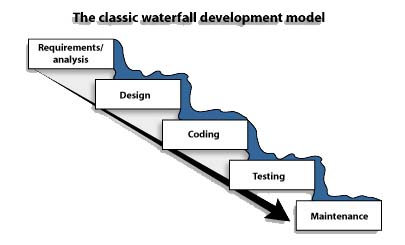
\includegraphics[width=10cm]{waterfall.jpg}
    \captionof{figure}{Obtenido de \cite{EmbededSystems}}
    \end{center}
\end{frame}

\begin{frame}
    \frametitle{Problemas con Waterfall}
    \begin{itemize}
        \item{Los requisitos cambian constantemetne.}
        \item{Dificil utilizar los recursos humanos eficientemente.}
        \item{Los errores cometidos en una etapa se amplifican
        en las siguientes etapas.}
        \item{Muy dificil corregir los errores, en especial
        cuando el sistema ya se termino. Ej. Xorg}
    \end{itemize}
\end{frame}

\begin{frame}
    \frametitle{Metodologias espirales}
    \begin{itemize}
        \item{El proceso de desarrollo se estructura mediante iteraciones.}
        \item{En cada iteraci\'on se repiten los mismos pasos.}
        \item{Cada iteraci\'on se retro-alimenta de las iteraciones anteriores.}
        \item{Las iteraciones se pueden ordenar segun diferentes criterios:
            \begin{itemize}
                \item{Enfocarse en un sub-sistema a la vez.}
                \item{En orden de riesgo.}
                \item{Implementar funciones claves primero, luego complementos.}
            \end{itemize}
        }
        \item{Con buenas practicas y un buen pipieline de desarrollo, los
        errores causados por cambios de requisitos se pueden mitigar.}
        \item{Existen varios modelos\cite{ScrumAgile}:
            \begin{itemize}
                \item{Extreme programming.}
                \item{Rational unified process (RUP)}
                \item{Scrum}
            \end{itemize}
        }
    \end{itemize}
\end{frame}

\begin{frame}
    \frametitle{Metodologias espirales}
    \begin{center}
    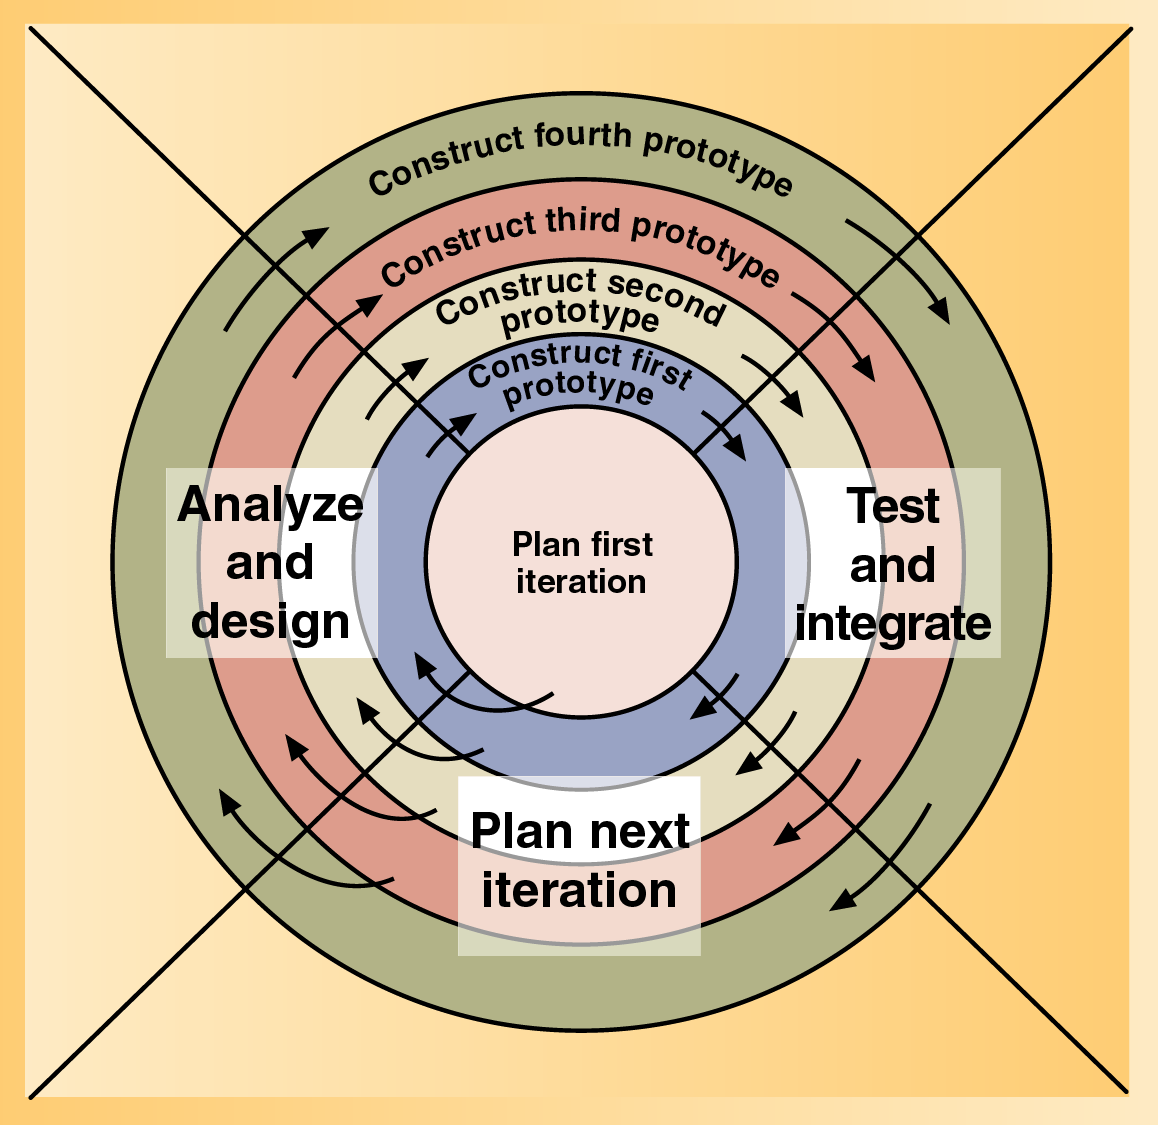
\includegraphics[width=7cm]{./spiral.jpg}
    \end{center}
\end{frame}

\begin{frame}
    \frametitle{Ventajas de las metodologias espirales}
    \begin{itemize}
        \item{Incl\'uyen el cambio como parte del proceso:
            \begin{itemize}
                \item{Aprender de iteraciones pasadas.}
                \item{Minimizan el riesgo y costo de introducir cambios.}
                \item{Minimizan la propagaci\'on de errores.}
            \end{itemize}
        }
        \item{Entregan valor temprano:
            \begin{itemize}
                \item{Satisfacer al cliente desde temprano.}
                \item{Reduce el riesgo de fallar.}
                \item{Se enfoca en la funcionalidad m\'as importante en cada etapa.}
            \end{itemize}
        }
        \item{En algunos casos, el cliente es parte del equipo:
            \begin{itemize}
                \item{Le permite al cliente dar retro-alimentaci\'on desde temprano.}
                \item{Mantiene al cliente informado.}
                \item{Facilita el dise\~no del sistema.}
            \end{itemize}
        }
        \item{Mayor utilizacion de recursos humanos:
            \begin{itemize}
                \item{Cada miembro del equipo puede trabajar en su campo durante todas las iteraci\'ones.}
                \item{No hay necesidad de esperar a que completen fases anteriores para trabajar.}
                \item{Todos los miembros tienen la misma importancia en todas las iteraciones.}
            \end{itemize}
        }
    \end{itemize}
\end{frame}

\begin{frame}
    \frametitle{Scrum}
    \begin{itemize}
        \item{Organiza el desarrollo en sprints de 2-4 semanas de duraci\'on.}
        \item{Los requisitos son capturados como historias en un backlog.}
        \item{Cada sprint debe producir un producto entregable.}
        \item{Antes de cada sprint debe haber una session de planeaci\'on.}
        \item{Los errores se van agregando al backlog seg\'un van siendo reportados.}
        \item{Requiere mucha transparencia y comunicaci\'on del equipo,
        para poder corregir y agendar errores. $\Rightarrow$ Encontrar errore es bueno.}
    \end{itemize}
\end{frame}

\begin{frame}
    \frametitle{Composici\'on de Scrum}
    \begin{itemize}
        \item{Ocupaciones:
            \begin{itemize}
                \item{Lider de proyecto}
                \item{Equipo}
                \item{Scrum master}
            \end{itemize}
        }
        \item{Ceremonias:
            \begin{itemize}
                \item{Planeaci\'on del sprint}
                \item{Revisi\'on del sprint}
                \item{Retrospectiva del sprint}
                \item{Reunion diaria}
            \end{itemize}
        }
        \item{Artefactos:
            \begin{itemize}
                \item{Backlog del sistema}
                \item{Backlog del sprint}
                \item{Burndown chart}
            \end{itemize}
        }
    \end{itemize}
\end{frame}

\begin{frame}
    \frametitle{Lider de proyecto}
    \begin{itemize}
        \item{A menudo referido como Product Manager (PM)}
        \item{Responsable de crear y priotizar la lista el backlog del sistema.}
        \item{Responsable de crear el sprint backlog en cada sprint.}
        \item{Interactua con los clientes y personas asociadas al sistema $\Rightarrow$ Refinar prioridades y requerimientos}
        \item{Asiste al equipo proporcionandole los recuros que necesiten para el desarrollo.}
        \item{Encargado de procesos administrativos.}
    \end{itemize}
\end{frame}

\begin{frame}
    \frametitle{Scrum master}
    \begin{itemize}
        \item{Supervisa el proceso:
            \begin{itemize}
                \item{Se asegura que los artefactos se utilizen adecuadamente.}
                \item{Se asegura que las ceremonias se lleven a cabo.}
                \item{Se asegura que todos los miembros participen debidamente.}
            \end{itemize}
        }
        \item{Asesora al equipo:
            \begin{itemize}
                \item{Ayuda al equipo a resolver problemas dificiles}
                \item{Ayuda a que exista comunicaci\'on efectiva en el equipo.}
            \end{itemize}
        }
        \item{El scrum master {\bf no} debe ser el lider del proyecto.}
    \end{itemize}
\end{frame}

\begin{frame}
    \frametitle{Equipo}
    \begin{itemize}
        \item{Generalmente peque\~no (2-7 personas) y centralizado.}
        \item{Multifuncional:
            \begin{itemize}
                \item{Personas con diferentes destrezas.}
                \item{Tiene todas las destrezas necesarias
                para desarrollar el producto.}
            \end{itemize}
        \item{Auto-organizado:
            \begin{itemize}
                \item{Cada miembro decide cuando esfuerzo poner en cada sprint.}
                \item{Las tareas se deben asignar seg\'un las habilidades,
                    no solo por la ocupaci\'on oficial.}
                \item{El equipo colabora para cumplir con sus tareas.}
            \end{itemize}
        }
        }
    \end{itemize}
\end{frame}

\begin{frame}
    \frametitle{Planeaci\'on del sprint}
    \begin{itemize}
        \item{Se realiza antes de comenzar cada sprint.}
        \item{Se refina el backlog del sistema:
            \begin{itemize}
                \item{Agregar o quitar requerimientos.}
                \item{Cambiar prioridad de requerimientos.}
            \end{itemize}
        }
        \item{Definir la meta del sprint.}
        \item{Seleccionar los requerimientos para avanzar a esa meta:
            \begin{itemize}
                \item{Refinar requerimientos $\Rightarrow$ crear tareas a partir de los requerimeintos.}
                \item{Estimar los recursos necesarios para dicho requerimiento.}
                \item{Crear el backlog para el sprint.}
            \end{itemize}
        }
        \item{Asignar tareas a los miembros del equipo.}
    \end{itemize}
\end{frame}

\begin{frame}
    \frametitle{Ejecuci\'on del sprint}
    \begin{itemize}
        \item{Cada miembro lleva a cabo su tarea asignada:
            \begin{itemize}
                \item{Dise\~no}
                \item{Programaci\'on:
                    \begin{itemize}
                        \item{Pair programming}
                        \item{Revisi\'on de codigo}
                        \item{Pruebas unitarias}
                        \item{Integraci\'on continua}
                    \end{itemize}
                }
                \item{Tareas administrativas:
                    \begin{itemize}
                        \item{Reuniones con los clientes.}
                        \item{Reportes.}
                        \item{Focus groups.}
                        \item{Varia seg\'un la empresa y el cliente}
                    \end{itemize}
                }
            \end{itemize}
        }
        \item{Una \emph{reunion diara}}
        \item{El sprint debe concluir con un sistema {\bf funcional}}
        \item{El equipo puede dejar tareas pendientes para el siguiente sprint.}
        \item{Los requisitos y ambito no cambian durante el sprint.}
    \end{itemize}
\end{frame}

\begin{frame}
    \frametitle{Reunion diaria}
    \begin{itemize}
        \item{Objetivos:
            \begin{itemize}
                \item{Mantener al equipo informado sobre los avances en el sprint.}
                \item{Exponer los problemas y obstaculos.}
                \item{Coordinar al equipo.}
            \end{itemize}
        }
        \item{Caracteristicas:
        \begin{itemize}
            \item{Corta, menos de 15 minutos $\Rightarrow$ parados}
            \item{Diaria, a la misma hora}
            \item{No es para resolver problemas.}
            \item{Pueden agendarse reuniones posteriores para discutir problemas.}
            \item{Ordenado: una persona presenta a la vez.}
        \end{itemize}
    }
    \item{Posible formato por miembro:
        \begin{enumerate}
            \item{¿Que hize ayer?}
            \item{¿Que hare hoy?}
            \item{¿Que obstaculos tengo?}
        \end{enumerate}
    }
    \end{itemize}
\end{frame}

\begin{frame}
\frametitle{Referencias}
\bibliography{../../Referencias/referencias}
\bibliographystyle{plain}
\end{frame}

\end{document}